\documentclass[a4paper, 12pt]{article}
\usepackage[utf8]{inputenc}
% \usepackage{fontspec}
\usepackage{graphicx}
\usepackage{hyperref}
\usepackage{changepage}
\graphicspath{ {images/} }
\usepackage[a4paper,left=1.5in,right=1in,top=1in,bottom=1in]{geometry}
\usepackage{times}
\usepackage{epsfig}
\usepackage{tikz}
\usetikzlibrary{positioning,shapes,fit,arrows}
\definecolor{myblue}{RGB}{56,94,141}
\usepackage{fancyhdr}
\usepackage{booktabs}
\usepackage{mathtools}
\usepackage{amsmath}
\usepackage{amssymb}
\usepackage{enumitem}
\usepackage{etoolbox}
%\apptocmd{\thebibliography}{\csname phantomsection \endcsname \addtocontentsline{toc}{chapter}{\bibname}}{}{}
\usepackage{caption}
\usepackage{float}
\floatstyle{boxed} 
\restylefloat{figure}
\pagestyle{fancy}
\fancyhf{}
% \fancyhead[LE,RO]{\footnotesize \center }
% \fancyfoot[CE,CO]{ \raggedright{\fontfamily{cmr}\select P:F-SMR-UG/08/R0}}
\fancyfoot[LE,RO]{\thepage}
\def\eg{\textit{e.g.}~}
\def\ie{\textit{i.e.}~}
\def\Eg{\textit{E.g.}~}
\def\etal{\textit{et al.}~}
\def\etc{\textit{etc.}~}
\def\ci#1{\textcircled{\resizebox{.4em}{!}{#1}}}
\renewcommand{\baselinestretch}{1}

\newcommand{\thr}[1]{\rotatebox[origin=c]{90}{#1}}
\newcommand{\tht}[2]{\begin{tabular}{@{}#1@{}}#2\end{tabular}}
\newcommand{\red}[1]{\textcolor{blue}{#1}}
\usepackage{hyperref}
\hypersetup{
    colorlinks=true,
    linkcolor=blue,
    filecolor=magenta,      
    urlcolor=cyan,
}
% \setsansfont{arial.ttf}
\usepackage[nottoc]{tocbibind} %Adds "References" to the table of contents
\begin{document}
 
\begin{titlepage}
    \begin{center}
        \vspace*{1cm}
        
        \large
                \textbf{\MakeUppercase{Pune Institute of Computer Technology}}
                \linebreak
        \textbf{\MakeUppercase{Dhankawadi, Pune}}
        \vspace{0.5cm}
                        \linebreak
                        \linebreak
        \MakeUppercase{DATA MINING AND WAREHOUSING  Mini-Project REPORT }
        \linebreak
        ON
        \linebreak
        \vspace{0.5cm}
        \large
        \\
        \textbf{\MakeUppercase{“Predicting Soccer Game Results using various models”}}
        \linebreak
        
        %\vspace{0.2cm}
        \textbf{SUBMITTED BY}
        \vspace{1cm}
        
        \begin{center}
        \begin{tabular}{ c c }
         Nachiket Erlekar & 41434 \\ 
         Ashay Koradia & 41429 
        \end{tabular}
        \end{center}
                
        \textbf{\large{Under the guidance of}}
        \linebreak
        Prof. Deepali Kadam
        \linebreak
      %  \vfill
        
        
        
        \vspace{0.8cm}
        

        
\includegraphics[scale=0.6]{pict.eps}   
        
        \Large
        DEPARTMENT OF COMPUTER ENGINEERING\\
%        \textbf{Pune Institute of Computer Technology}    
%        \textbf{Dhankawadi, Pune}
%        \linebreak
        \textbf{Academic Year 2020-21}
        
    \end{center}
\end{titlepage}
\pagebreak

\newpage
\tableofcontents
\newpage
\pagenumbering{arabic}
\begin{center}
    \section{Problem Statement}
\end{center}
\par Consider a labeled dataset belonging to an application domain. Apply suitable data preprocessing steps such as handling of null values, data reduction, discretization.  For prediction of class labels of given data instances, build classifier models using different techniques (minimum 3), analyze the confusion matrix and compare these models. Also apply cross validation while preparing the training and testing datasets.

\newpage
\begin{center}
    \section{Abstract}
\end{center}
Classification is a form of data analysis that extracts models describing importantdata classes.  Such models, called classifiers, predict categorical (discrete, unordered)class labels.  For example, we can build a classification model to categorize bank loanapplications as either safe or risky. Such analysis can help provide us with a better un-derstanding of the data at large. In this project we use multiple classification models toanalyse the outcome of Soccer game played between various teams. Use apply suitabledata preprocessing steps.We then compare performance of classification models to findwhich one is the best
\newpage
\begin{center}
    \section{Hardware and Software Requirements}
\end{center}
\subsection{Hardware Requirements}
\begin{enumerate}
    \item 500 GB HDD
    \item 4GB RAM
    \item Monitor
    \item Keyboard
\end{enumerate}

\subsection{Software Requirements}
\begin{enumerate}
    \item 64 bit Open Source Operating System like Ubuntu 18.04
    \item Python 3
    \item Google Colab
    \item Different Libraries
    \item Libararies like sklearn, pandas, matplotlib
\end{enumerate}
\pagenumbering{arabic}
\newpage
\begin{center}
\section{INTRODUCTION}
\end{center}
\hspace{1cm}
\par
We have been provided with the data regarding various aspects of the home team, the opposition team and their supporters for a number of Soccer games.
\\
The Data fields are\\
\begin{enumerate}
    \item Id $-$ Unique id given to each game.
    \item game\_seq $-$ Sequence of the game in the history of FIH (International Soccer Federation).
    \item season\_end $-$ Year in which the corresponding season ended.

    \item date $-$ Date on which the game was played.

    \item season\_game\_seq $-$ Sequence of the game in the corresponding season.
    \item playoff $-$ Whether the game is a playoffs game.

    \item team\_id $-$ Unique id for the home team.

    \item Elo $-$ Elo rating for the home team before the game.

    \item opp\_team\_id $-$ Unique id for the opposition team.

    \item opp\_Elo $-$ Elo rating for the opposition team before the game.

    \item win\_equivalent $-$ Equivalent number of wins for the home team in a season.

    \item bet\_ratio $-$ Fraction of bets placed on the home team.
    \item home\_crowd $-$ Number of supporters for the home team.
    \item opp\_crowd $-$ Number of supporters for the opposition team.
    \item total\_crowd $-$ Total number of attendees for the game.
    \item game\_result $-$ Win or loss for the home team (Win - 1, Loss - 0).
\end{enumerate}

The train set contains 45000 records while the test set contains 13107 records.We drop the date column from our analysis. 
The null entries are as follows
\begin{table}[h]
    \centering
    \begin{tabular}{|c|c|}
    \hline
    Attribute & Null Count\\
    \hline
    Elo & 9197\\
    \hline
    opp\_Elo & 7006\\
    \hline
    win\_equivalent & 12263\\
    \hline
    \end{tabular}
    \caption{Null Counts}
    \label{tab:my_label}
\end{table}
\par We fill the null Elo and opp\_elo entries with the mean value of Elo and opp\_Elo attribute respectively i.e. 1501.184 & 1501.837

\newpage
\begin{center}
\section{OBJECTIVE}
\end{center}
\begin{itemize}
   \item To understand data preprocessing
    \item To perform classification on dataset and predict labels for test dataset.
\end{itemize}


\newpage
\begin{center}
\section{Scope}
\end{center}

We select dataset of soccer games of various seasons. We try to apply many models and compare which one is the best model amongst them.

\newpage
\begin{center}
    \section{System Architecture}
\end{center}
\par
\begin{figure}[h]
    \centering
    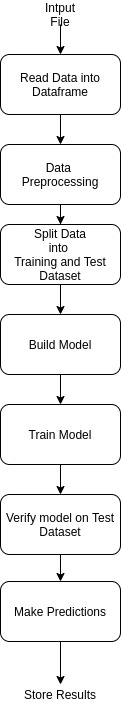
\includegraphics[scale=0.71]{DA-SA.jpg}
    \caption{System Architecture}
\end{figure}

\newpage
\begin{center}
\section{Test Cases}
\end{center}
\begin{center}
    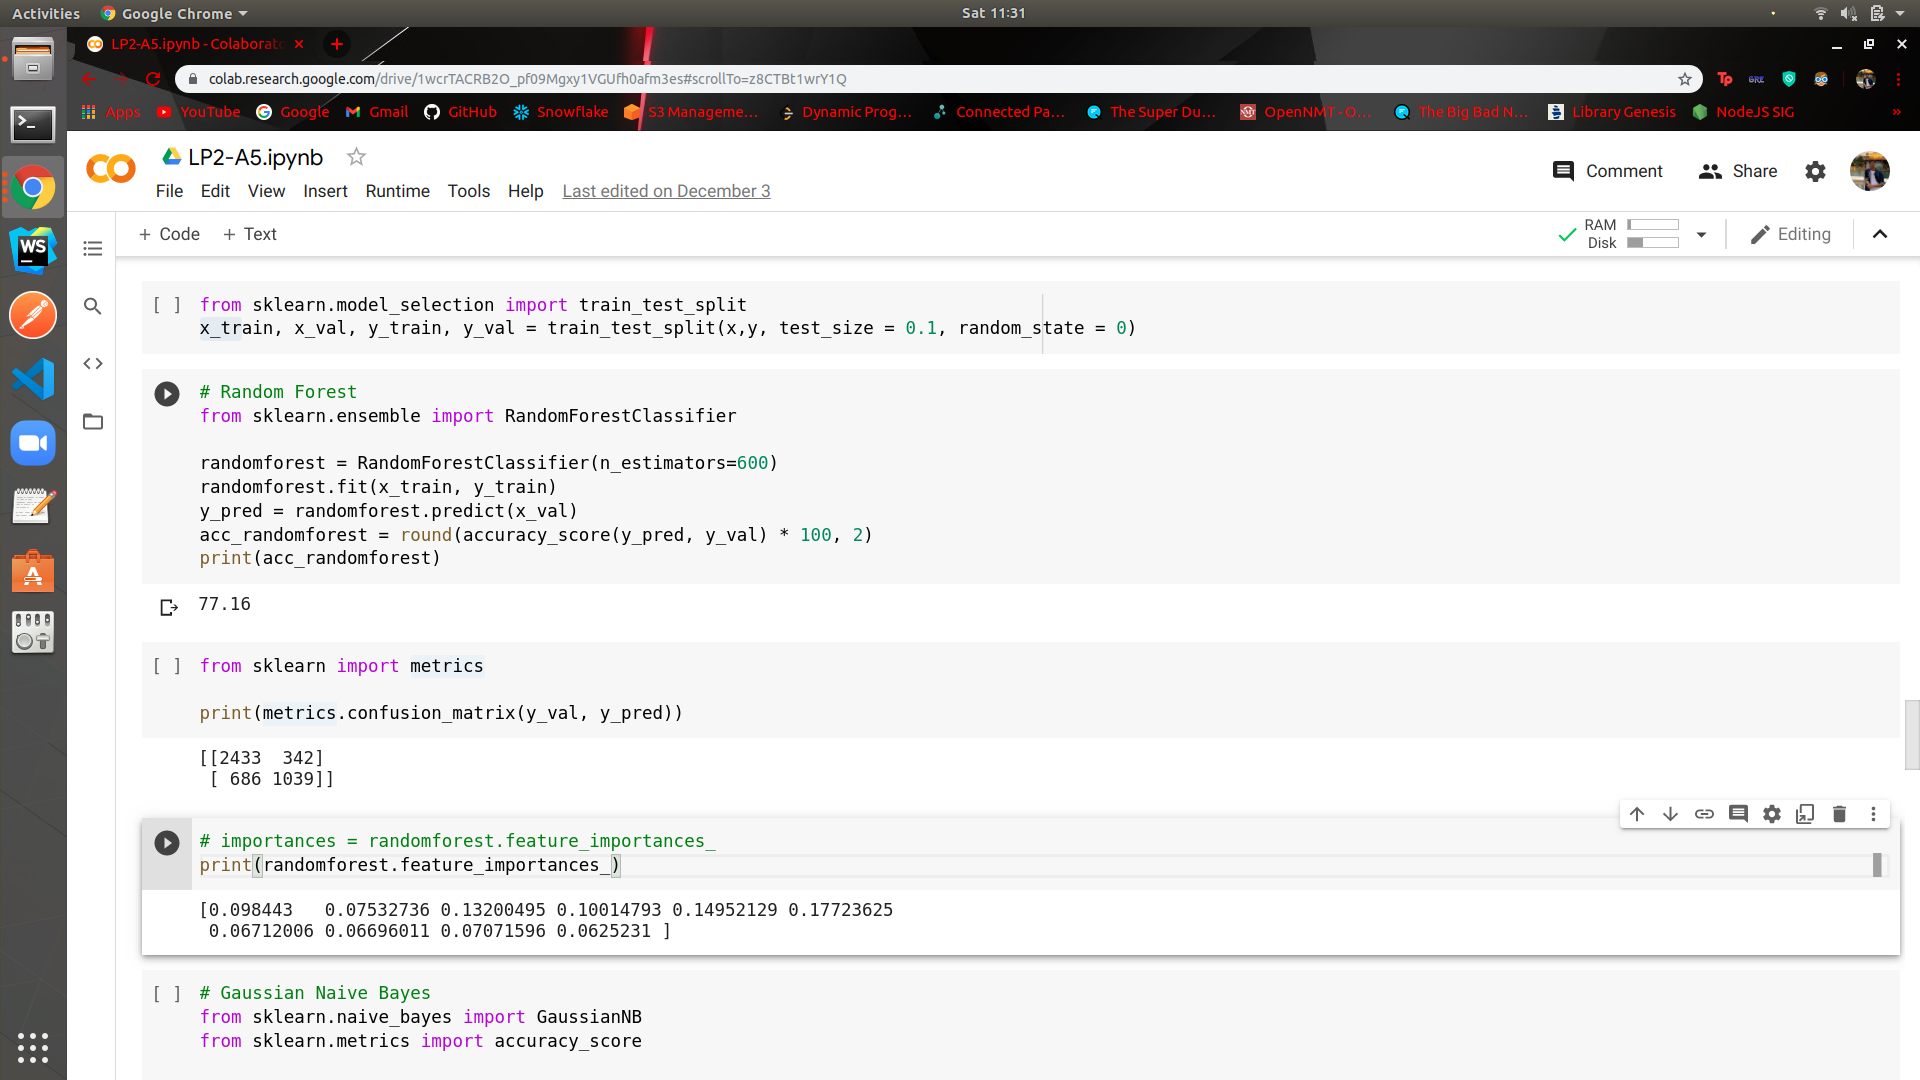
\includegraphics[width=\linewidth]{RF.png}
     \captionof{figure}{Output for Random Forest Classifier}
\end{center}
\begin{center}
    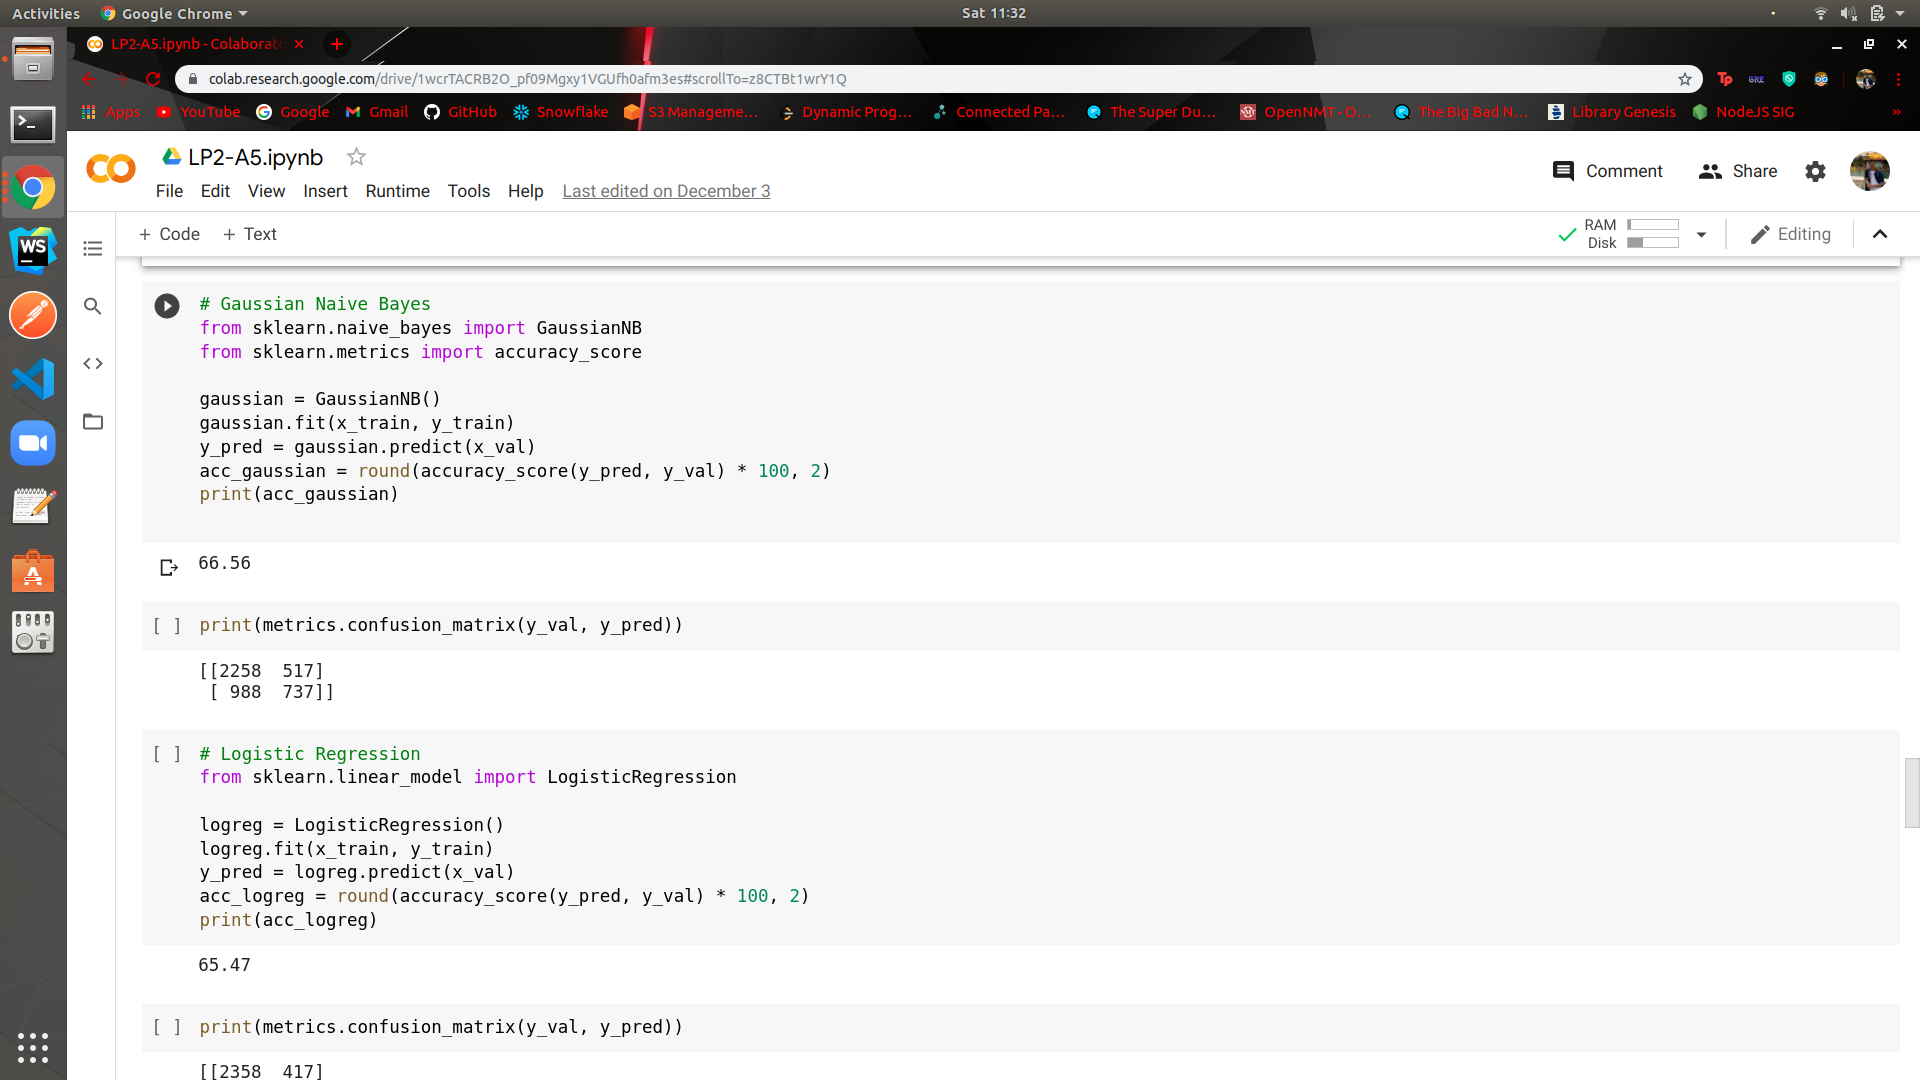
\includegraphics[width=\linewidth]{GNB_LR.png}
     \captionof{figure}{Output for GaussianNB and Logistic regression classifier}
\end{center}
\begin{center}
    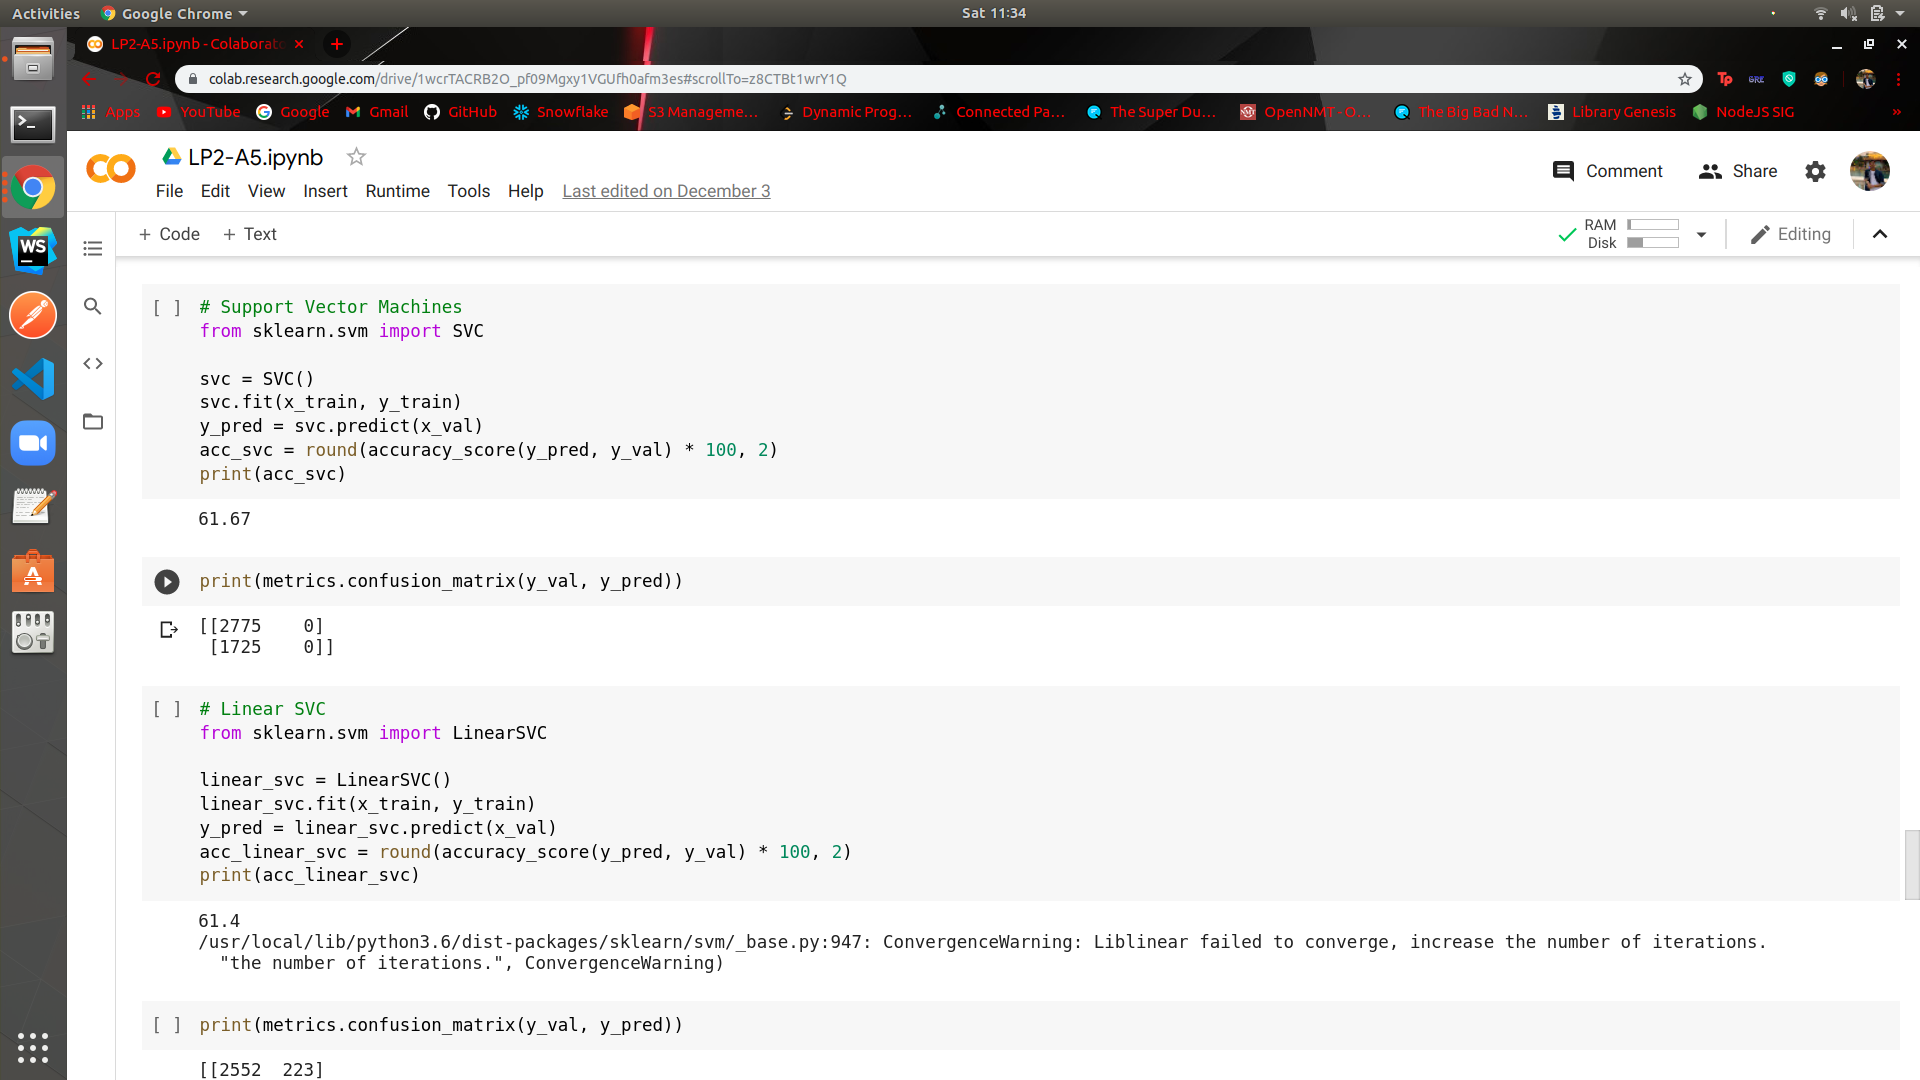
\includegraphics[width=\linewidth]{SVC_LSVC.png}
     \captionof{figure}{Output for SVC and Linear SVC}
\end{center}
\begin{center}
    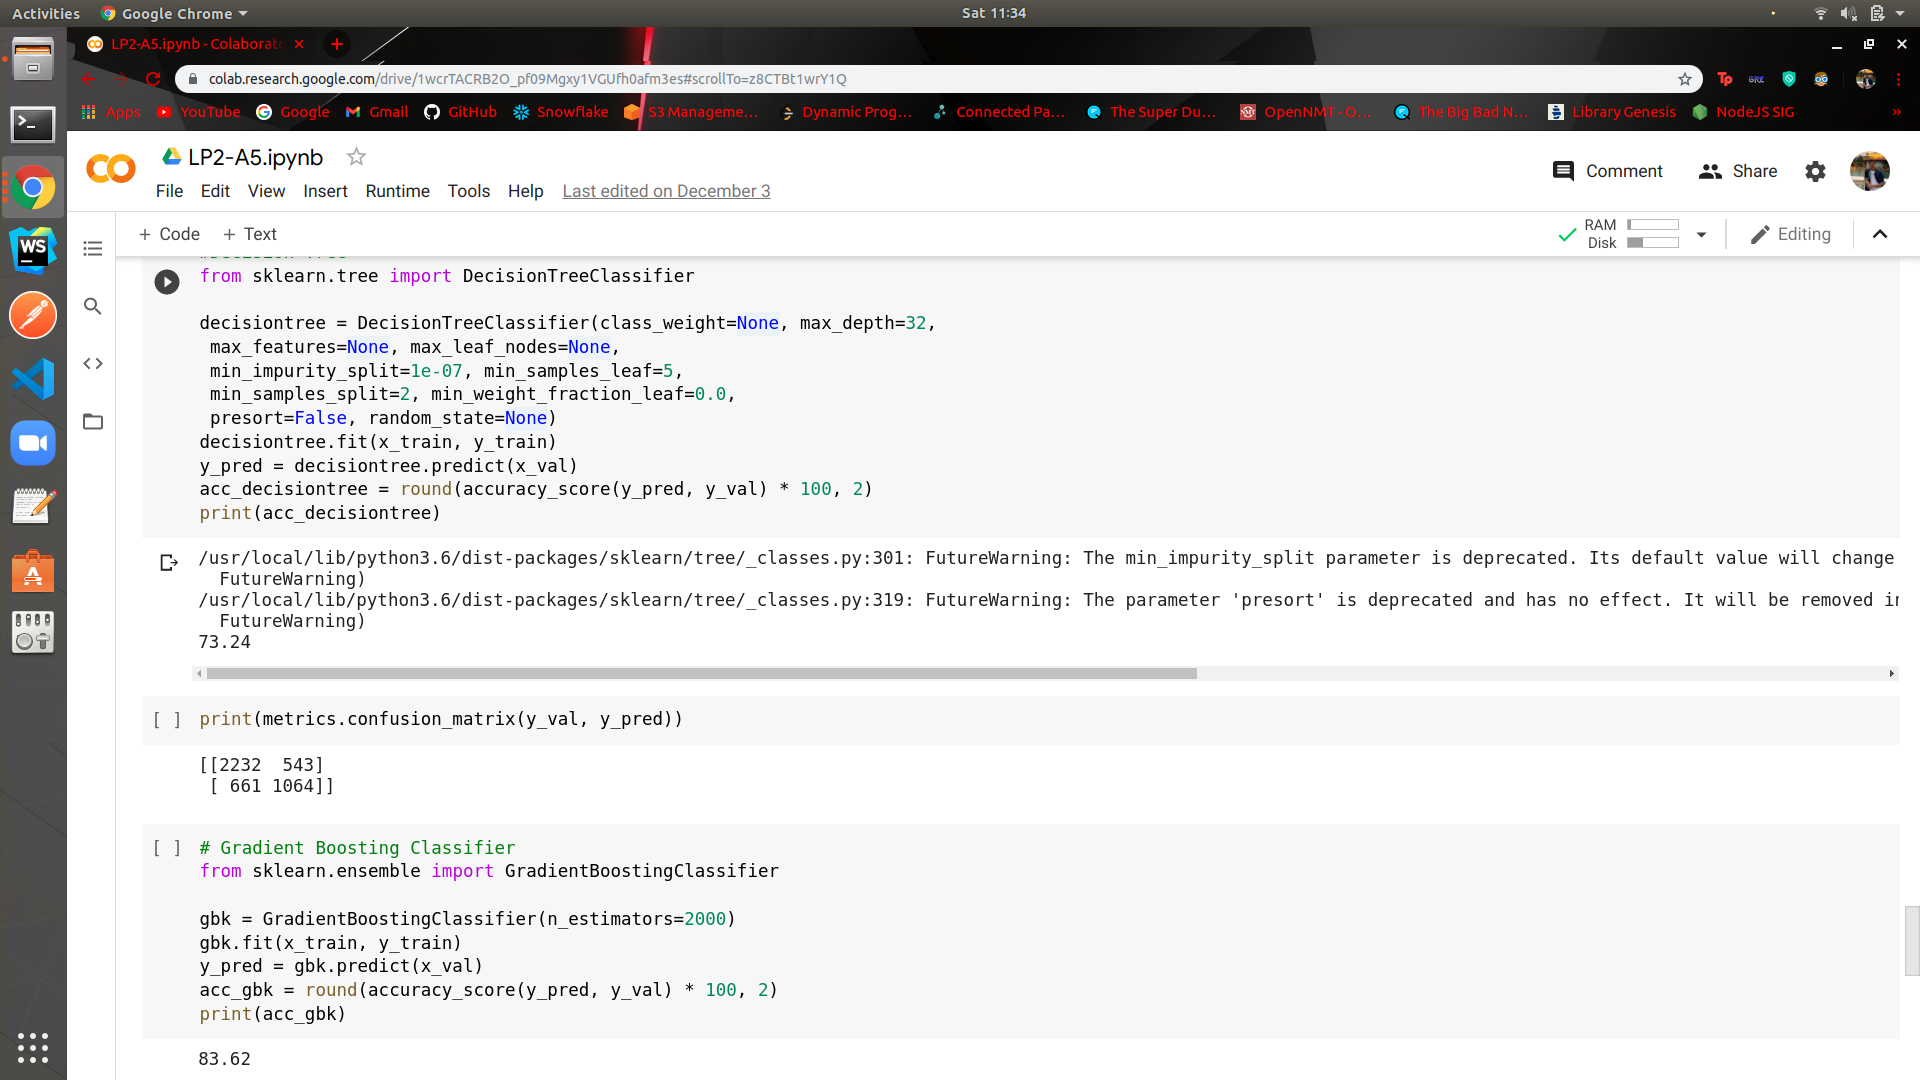
\includegraphics[width=\linewidth]{DT_GB.png}
     \captionof{figure}{Output for Decision tree and Gradient boosting classifier}
\end{center}


\newpage
\begin{center}
\section{Result}
\end{center}
\par 
The Accuracy for Various models are:
\begin{table}[h]
    \centering
    \begin{tabular}{|c|c|}
    \hline
         Model & Accuracy \\
    \hline
         DecisionTree & 73.24\\
    \hline
    RandomForest & 77.16\\
    \hline
    GaussianNB & 66.56\\
    \hline
   
    LogisticRegression & 65.47\\
    \hline
    SVC & 61.67 \\
    \hline
    LinearSVC & 61.4 \\
    \hline
    GradientBoostingClassifier & 83.62 \\
    
    \hline
    \end{tabular}
    \caption{Accuracy of vaious Models}
\end{table}
\par  We see that Gradient Boost Classifier gives the best score. We then use this model to perform training and testing of the model. After training, the model gives an accuracy of 83.62  \%.

\begin{center}
    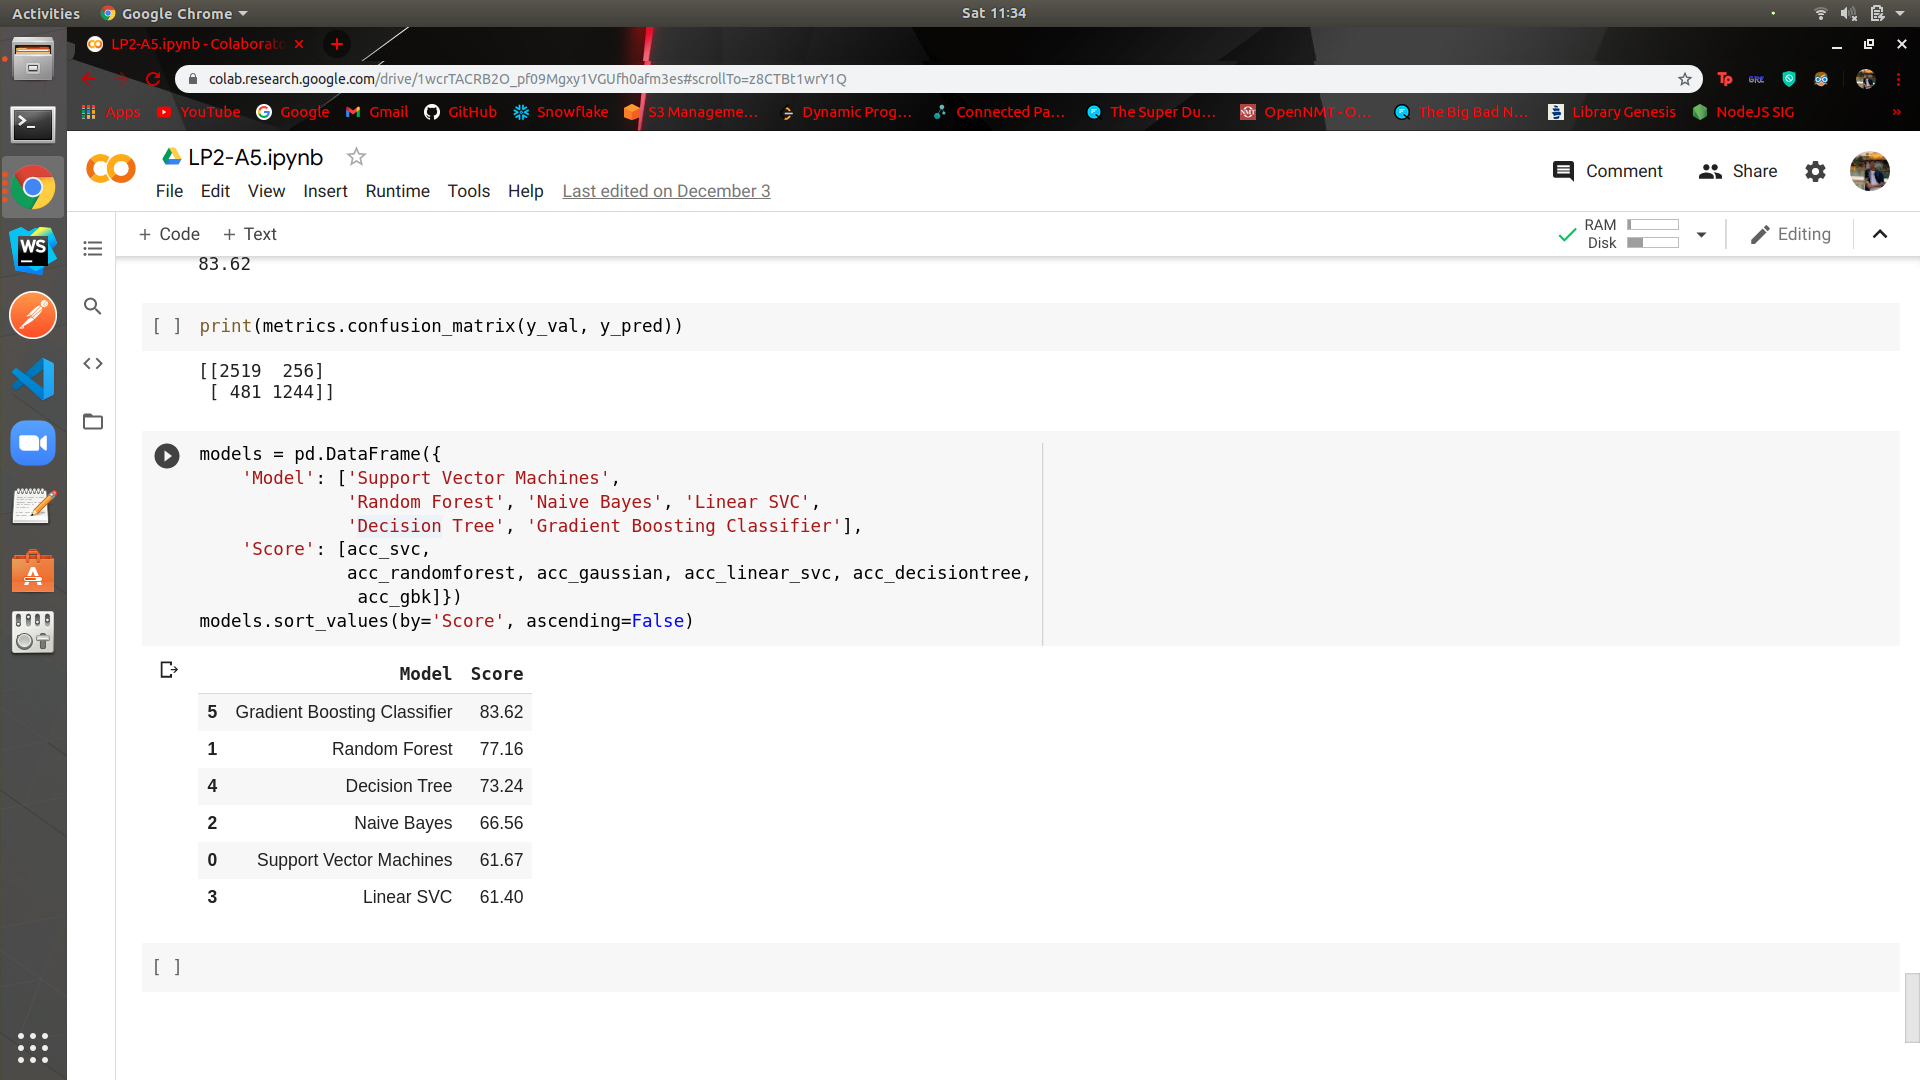
\includegraphics[width=\linewidth]{Comparison.png}
     \captionof{figure}{Comparison of various models}
\end{center}
\newpage
\begin{center}
\section{Conclusion}
\end{center}
We have analysed the Soccer game dataset and performed data pre-processing steps.We have experimented multiple classification models and found out the best performer amongt them. 
We presented classification of soccer game results to predict the win/loss using Gradient Boost Classifier. We report a classification accuracy of 83.62%
\newpage
\begin{thebibliography}{1}
\bibitem{dataset}
    \texttt{https://scikit-learn.org/stable/modules/generated/sklearn.ensemble.RandomForestClassifier.html}
\bibitem{sklearn}
    \texttt{https://scikit-learn.org/stable/modules/generated/sklearn.ensemble.GradientBoostingClassifier.html}
    \bibitem{sklearn}
    \texttt{ https://www.kaggle.com/c/datawiz19round1/data}
   
\end{thebibliography}
\end{document}
